\setcounter{secnumdepth}{-1}

\chapter{Synchronization errors}

\section{Description}

Because the receiver and transmitter are not at the same location, the carrier frequencies and the samplers at TX and RX will have a different phase and due to the inaccuracies of the oscillator, the frequencies will also be slightly different. \\
This is summarized in 4 effects:
\begin{itemize}
    \item \textbf{Carrier frequency offset (CFO)}: The difference in the carrier frequencies at TX and RX ($=\Delta \omega$). It will add ISI as the RRC are not anymore matched and a linearly increasing phase shift will appear.
    \item \textbf{Phase offset}: The difference between the phase of the carrier signal at TX and RX.
    \item \textbf{Sampling frequency offset (SFO)}: The difference in the sampling frequencies at TX and RX.
    \item \textbf{Time shift}: The difference in the timing of the samples at TX and RX.
\end{itemize}

\section{Implementation}

\subsection{CFO}
The CFO implementation is done by multiplying the signal with a complex exponential $e^{j2\pi \phi_{\text{ppm}}f_c t}$. The phase offset is added to the CFO. It is defined in ppm (part per million) where the ppm value is $\frac{\Delta\omega}{f_c} 10^{-6}$. \\
Figure \ref{fig:CFO_BER} shows the BER curves with different CFO values. In order to have useful results, the linear phase shift is removed right after the second RRC filter. This allows to only keep the effect of ISI on the BER curve.

\begin{figure}[H]
    \centering
    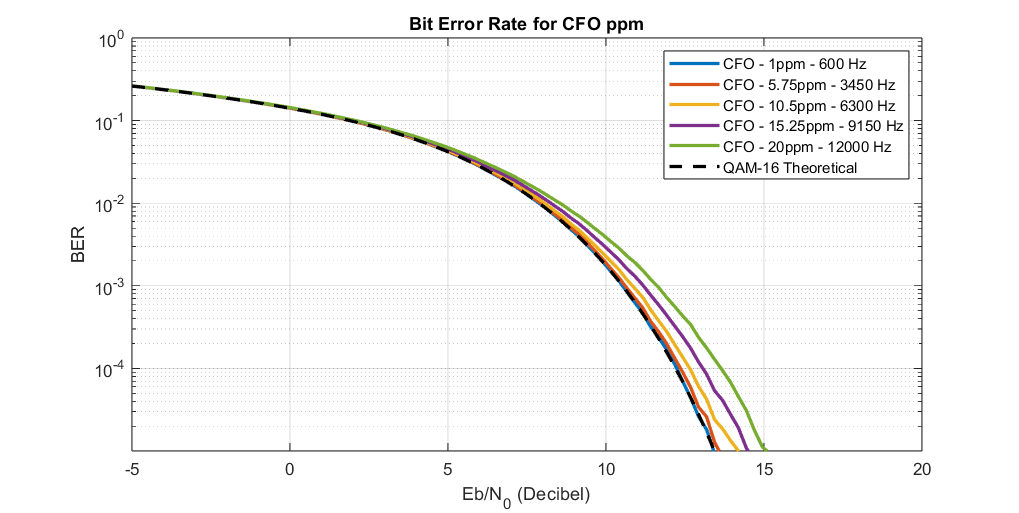
\includegraphics[width=0.8\textwidth]{CFO_ppm.png}
    \caption{BER with different CFO values}
    \label{fig:CFO_BER}
\end{figure}

Figure \ref{fig:CFO_const} shows the effect of CFO on the symbol constellation for QAM-16. It is here plotted without any noise and with parameters that allow us to see the line phase shift of the symbols. \\

\begin{figure}[H]
    \centering
    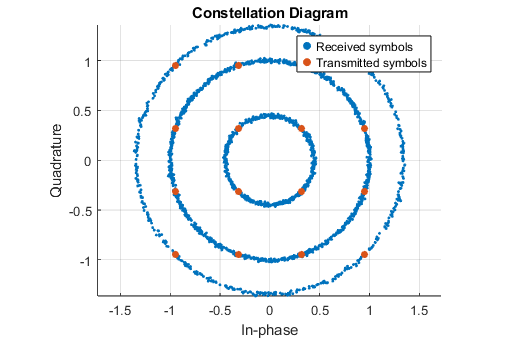
\includegraphics[width=0.8\textwidth]{constellation_CFO.png}
    \caption{Constellation before and after CFO}
    \label{fig:CFO_const}
\end{figure}

\subsection{Phase offset}
The same is done for the phase offset where the exponential is simply $e^{j\phi}$ where $\phi$ is chosen once at the begining of the simulation. \\

The effect of the phase offset is only visible on the constellation plot (figure \ref{fig:phaseOffsetConst}) where every point is rotated by a fixed angle (whereas CFO rotated the symbols linearly with time). \\

\begin{figure}[H]
    \centering
    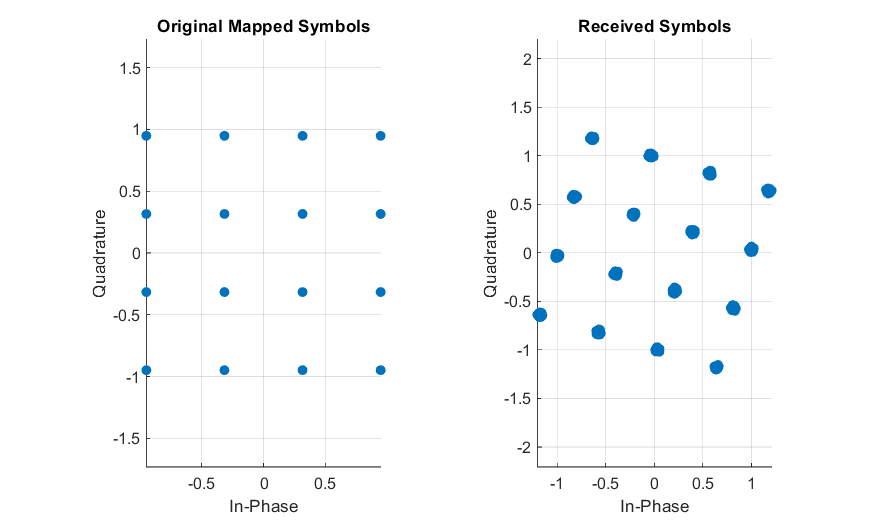
\includegraphics[width=0.8\textwidth]{constellation_carrier_offset.png}
    \caption{Constellation before and after phase offset}
    \label{fig:phaseOffsetConst}
\end{figure}

On a BER curve (figure \ref{fig:BER_PO}), the phase is not visible as from the errors originating from the phase offset are either on every symbol or on none and this is why the error does not depend anymore on $E_b/N_0$. \\

\begin{figure}[H]
    \centering
    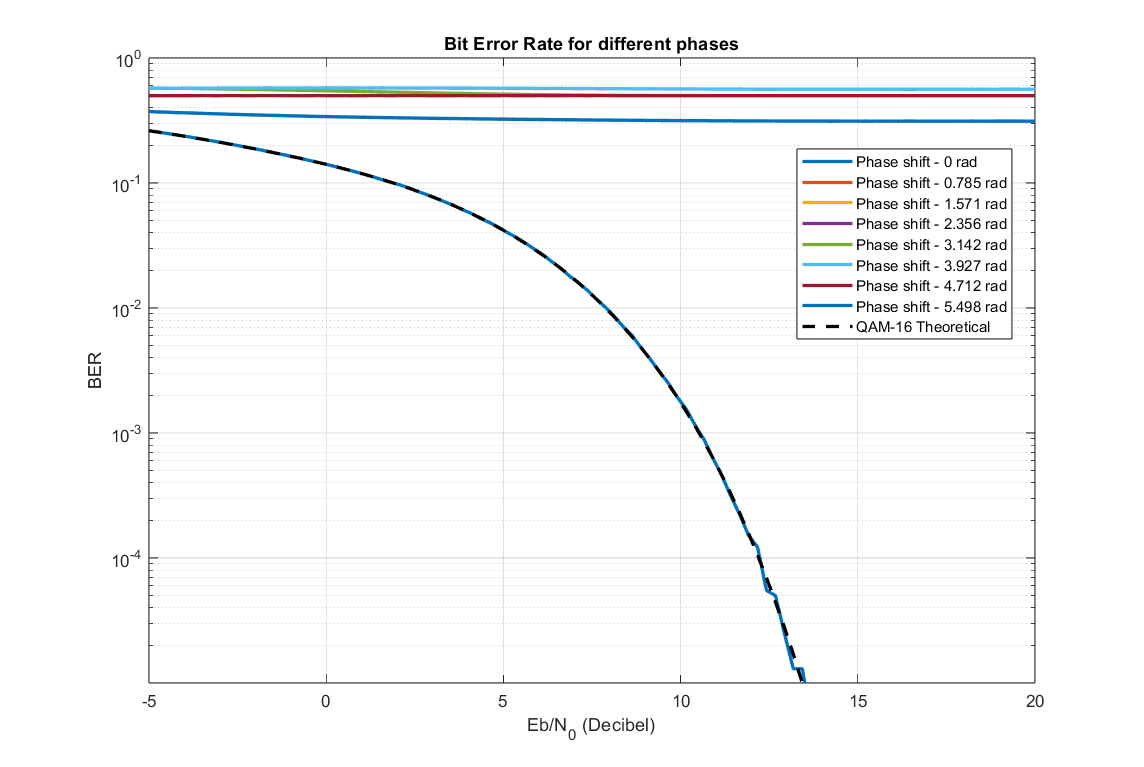
\includegraphics[width=0.8\textwidth]{BER_PO.png}
    \caption{BER with phase offset}
    \label{fig:BER_PO}
\end{figure}

\subsection{SFO}
The SFO is neglected in the simulation as it would need some interpolation and more complex computations. \\

\subsection{Time shift}
The time shift is implemented by simply shifting the samples in the array with an oversampling factor that is large enough. \\
A larger time shift will increase the BER as the samples will be taken at the wrong time. For sufficiently low values, it will still behave as a "classical" BER curve but from some point, there is just no more correlation between the measured sample and the received one and the BER tends to a $0.5$ line, as shown in figure \ref{fig:BER_TS}. \\

\begin{figure}[H]
    \centering
    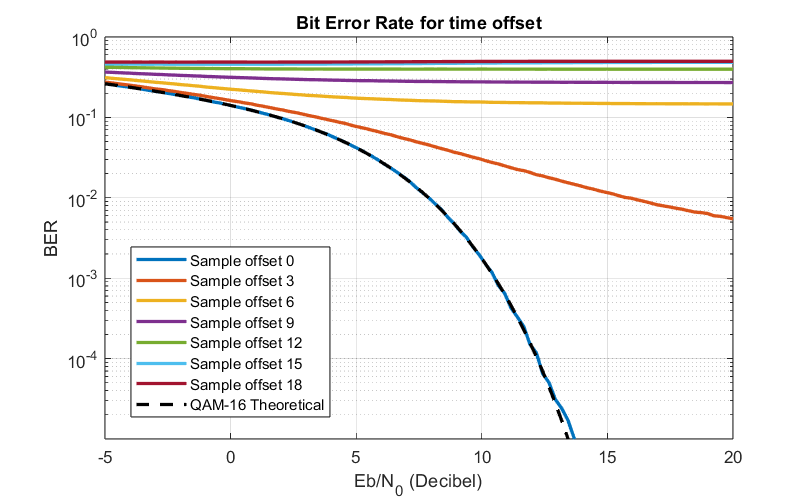
\includegraphics[width=0.8\textwidth]{BER_TS.png}
    \caption{BER with time shift}
    \label{fig:BER_TS}
\end{figure}

\subsection{Choice of $E_{b}/N_{o}$}
Securing a SNR high enough to ensure a remaining acceptable time error after Gardner algorithm implementation
 (2 percents of the symbole rate) is a necessary condition to fulffill.\\
The impact on the BER can be seen on the graph below - figure \ref{fig:time_shift_error_SNR}.
In our case, for a symbol rate of 5MHz, the SNR should be above 4dB - 5dB and will be used in our simulation.
Morevover, this SNR allows us to achieve, once the frame synchronisation implemented, a remaining carrier frequency offset
of 2 ppm which is very close from the BER performance we can get without CFO - figure \ref{fig:carrier_shift_error_SNR}.


\begin{figure}[H]
    \centering
    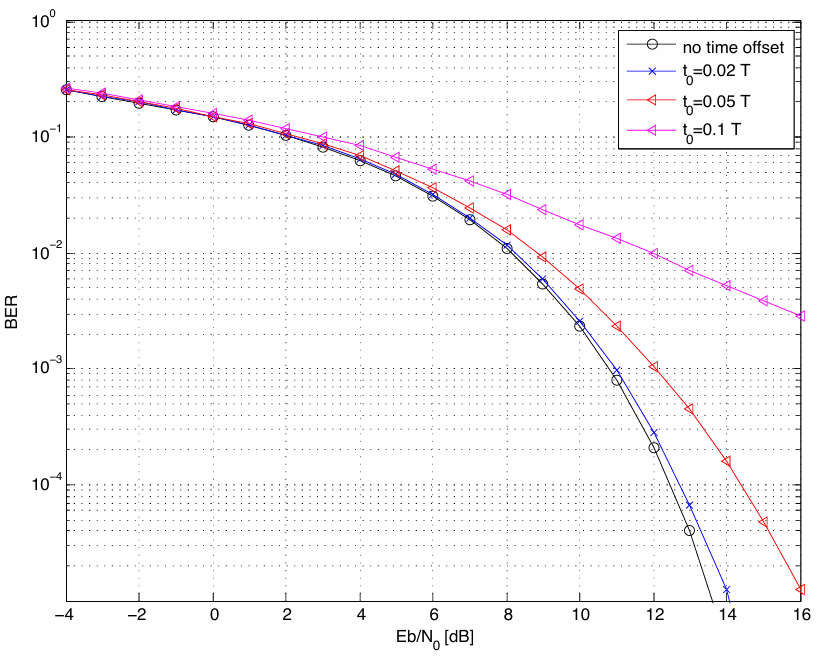
\includegraphics[width=0.8\textwidth]{time_shift_error_SNR.png}
    \caption{Impact of time shift on bit error rate}
    \label{fig:time_shift_error_SNR}
\end{figure}

\begin{figure}[H]
    \centering
    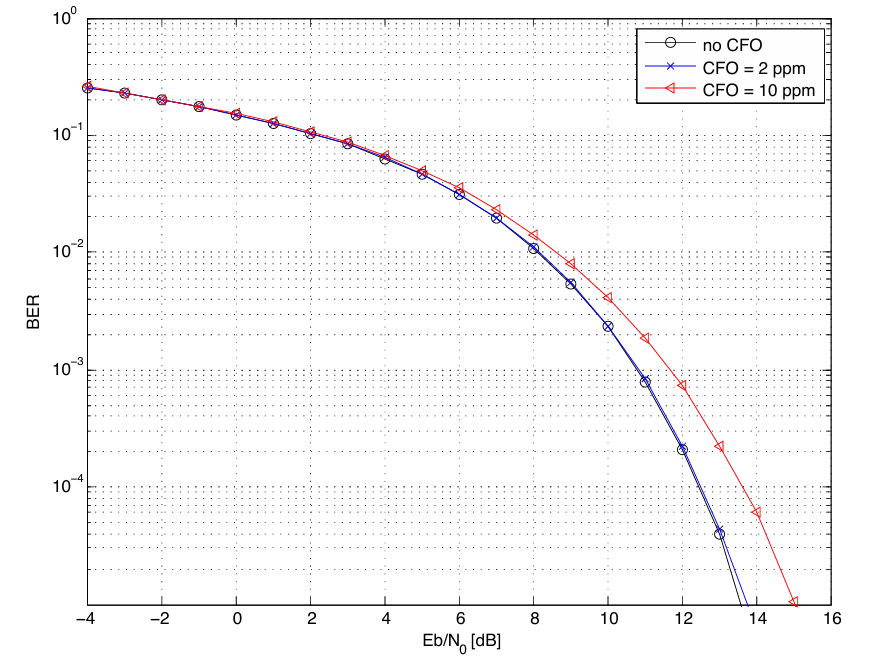
\includegraphics[width=0.8\textwidth]{carrier_shift_error_SNR.png}
    \caption{Impact of carrier frequency offset on bit error rate}
    \label{fig:carrier_shift_error_SNR}
\end{figure}

\subsection{Length of the pilot and the data sequence}

Another condition to successfully implement the frame synchronisation algorithm and secure a remaining 
CFO of 2 ppm, for a SNR of 4-5dB, is to ensure to get:
\begin{itemize}
    \item A preamble with a large enough number of symbols (N>20).
    \item Cross-correlation sub-windows which are enough separated (K>8).  
\end{itemize}

\section{Correction}

\subsection{Synchronisation error correction order}

The main bottleneck of the synchronisation error correction is the combination of the time shift error and
 the carrier frequency error.
This error combination leads us to find a algorithm which correct an error whithout being affected by the other error.
Gardner algorithm is fulfilling this condition.  It allows to correct the time shift error being robust to any realistic CFO error.
Once the time shift error is corrected, the second algoritm can be implemented and detect/estimate the frequency shift introduced by the CFO.\newline

The results of our Matlab code for different time shifts and different weigthed coefficient \textbf{k} can be seen below.

\begin{figure}[H]
    \centering
    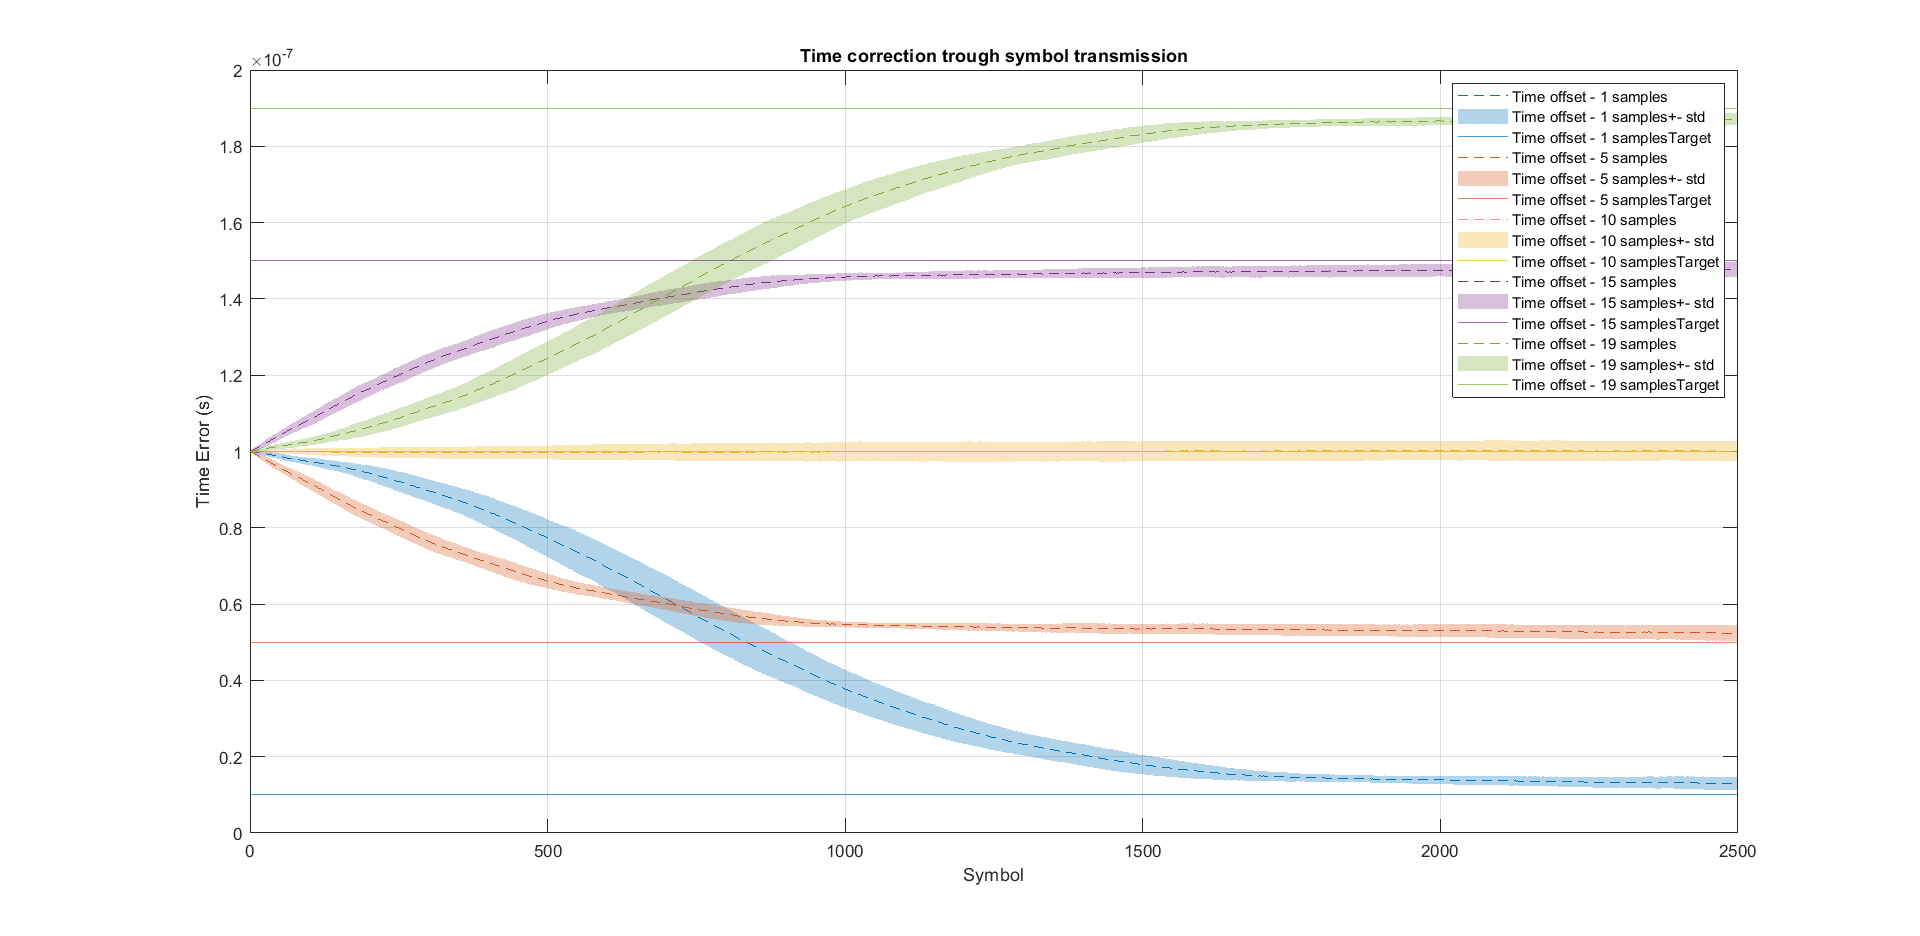
\includegraphics[width=0.8\textwidth]{Gardner_time_error_correction.png}
    \caption{Time error correction results from our Matlab code}
    \label{fig:Gardner_time_error_correction}
\end{figure}

\begin{figure}[H]
    \centering
    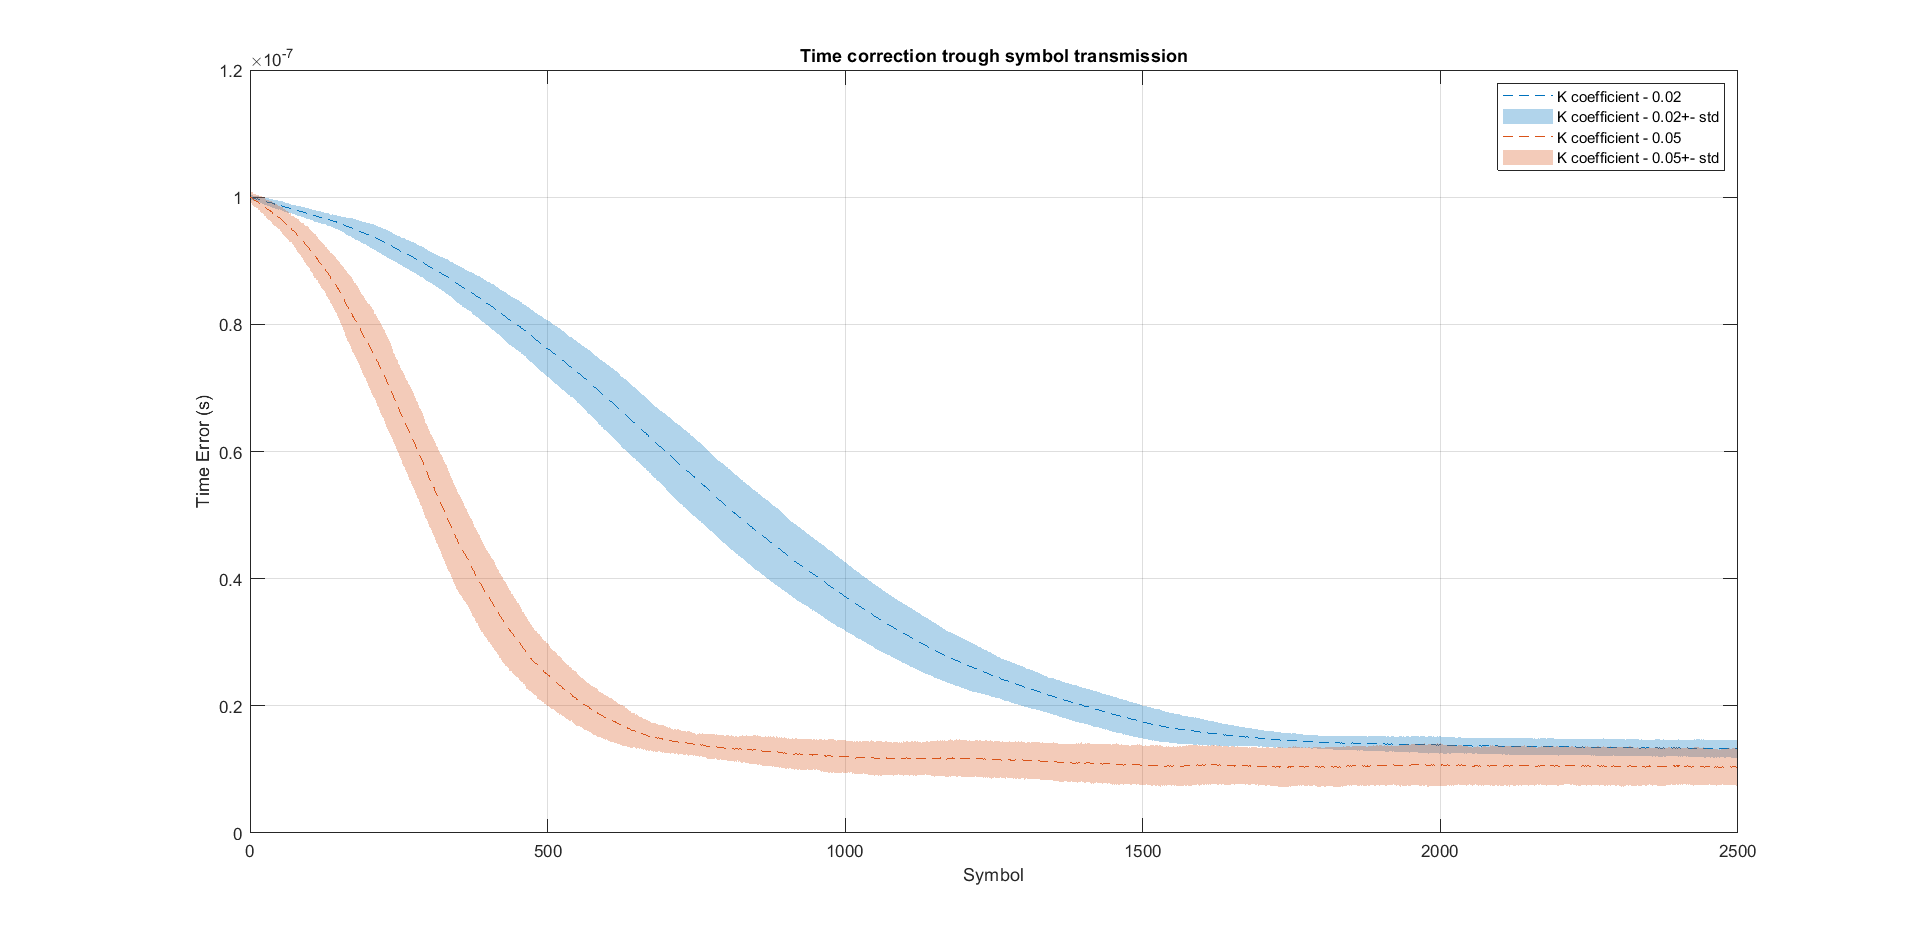
\includegraphics[width=0.8\textwidth]{Gardner_weigthed_coefficient.png}
    \caption{Time error correction results with different weighted coefficient from our Matlab code}
    \label{fig:Gardner_weigthed_coefficient}
\end{figure}

It is also interesting to mention that the Gardner algorithm is a \textbf{continuous} error correction - which means that
the time shift error is corrected along the symbol stream sending.\\
In the other hand, The frame synchronisation is a correction done by analyzing a \textbf{window} of symbols.

\subsection{CFO robustness of the Gardner algorithm}

To understand why the Gardner algorithm is robust to CFO, we would need to analyze mathematicall the algorithm.

\begin{equation*}
    \epsilon_{n+1} = \epsilon_{n} - \frac{2k}{T} R[y_{\epsilon_{n}}[n-\frac{1}{2}](y_{\epsilon_{n}}^{*}[n] - y_{\epsilon_{n-1}}^{*}[n-1])]
\end{equation*}

By taking a close look to the equation, we can observe that the error is corrected by taking 2 adjacent symbols (which is why the algorithm is
continuous). This specificity limits the effect of a phase shift as limited between 2 neighboring symbols.

\subsection{Differential cross-correlation}

Let's have a closer look to the cross correlation equation to grasp the intuition behind the need to use the differential cross-correlation.

\begin{equation*}
    \sum_{l}{y^{*}_{n+l}a_{l}} = \sum_{l}{I^{*}_{n+l}a_{l}e^{-j\phi_{o}}e^{-j\Delta w(n+l)T}}
\end{equation*}

We can observe that the CFO term is increasing with \textbf{n} resulting to a cross correlation equals to 0 even if the preamble is fitting
the window.

Therefore, the idea behind the usage of the differential cross correlation is to remove the dependency of the phase shit with \textbf{n}.
This idea leads to modify the equation and multiply the correlation between $y$ and $a$ with its complex conjudgate term. Indeed the exponential 
terms are cancelling and remains an exponential dependent on k, the window division term.
Therefore, by computing the differential cross correlation, the calculation will result to a peak once the preamble will match with the synchronisation
 window, function of $e^{-j\Delta wk}$ and 0 in the other cases.
 
To reply to the sub-question quoting "Isn’t interesting to start the summation at k = 0 (no time shift)?", of course the reply is no as explained above.

The robustness of the gardner algorithm implemented in our Matlab code can be seen in \ref{fig:Gardner_CFO_robustness}

\begin{figure}[H]
    \centering
    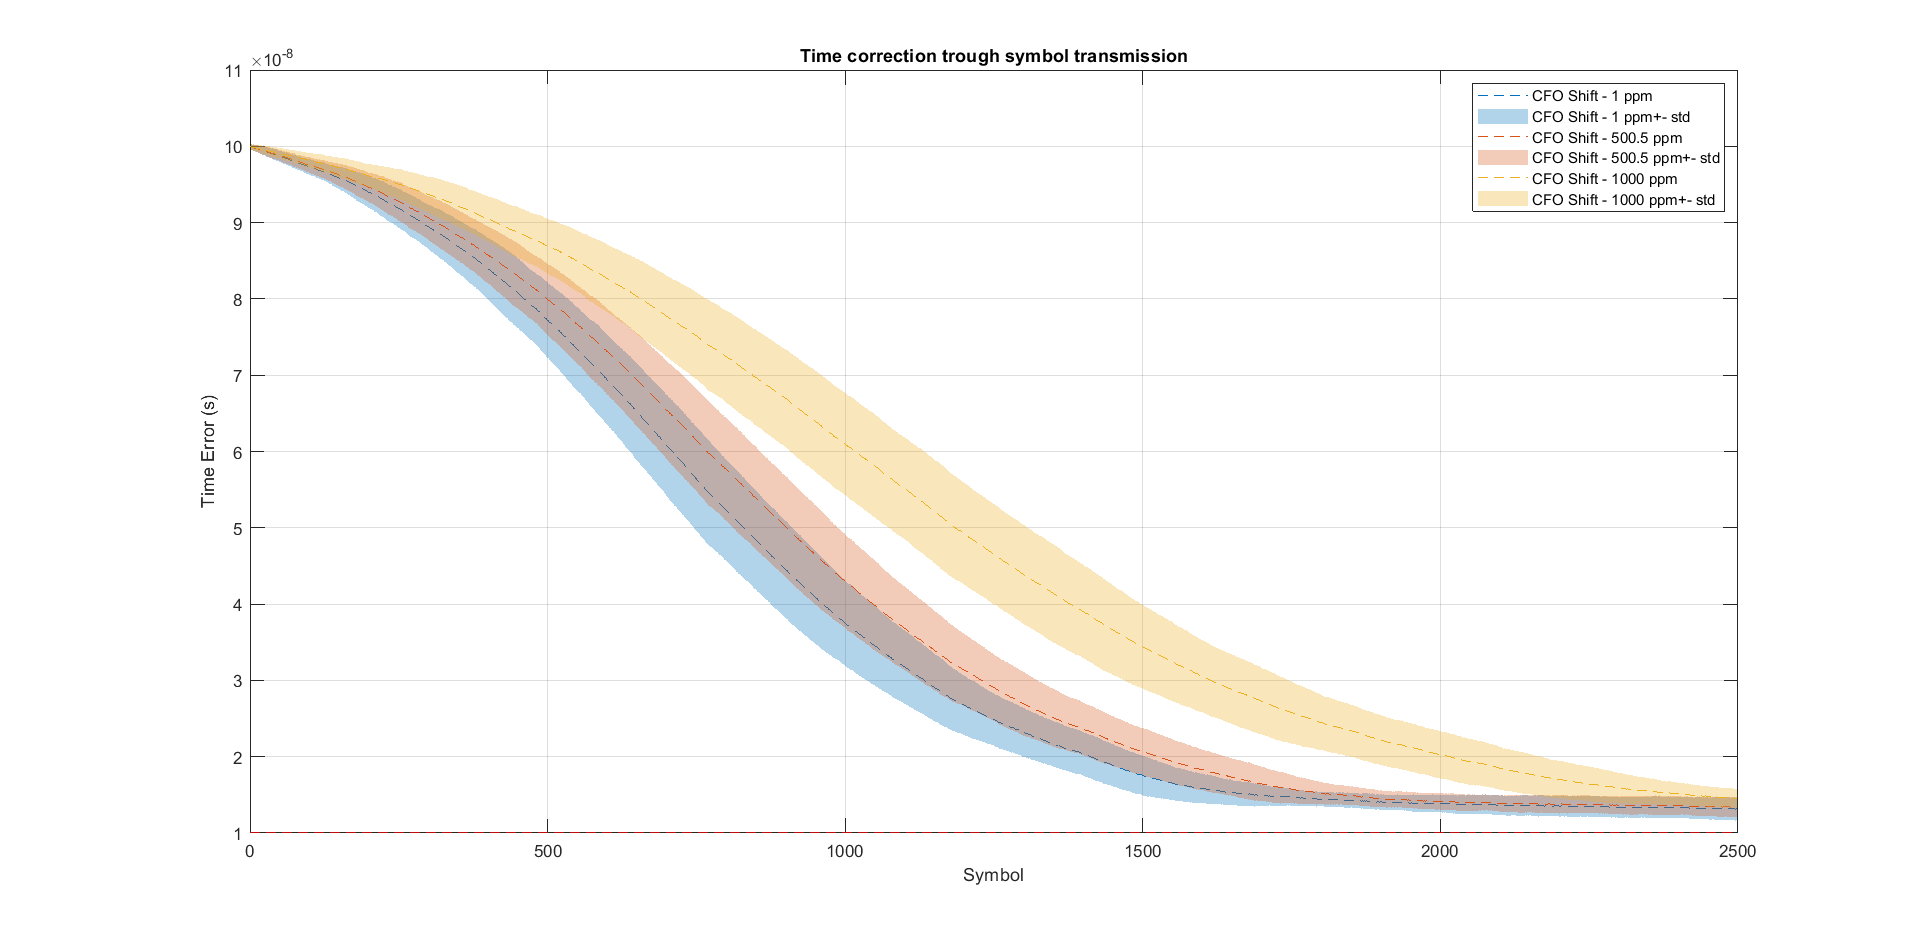
\includegraphics[width=0.8\textwidth]{Gardner_CFO_robustness.png}
    \caption{CFO robustness results from our Matlab code}
    \label{fig:Gardner_CFO_robustness}
\end{figure}

\subsection{Optimal criteria}

To summarize, to have a perfect frame synchronisation which means to have a frame time arrival standard deviation equals to 0 for a realistic CFO
error and a remaining time error of 2 percents at the end of Gardner module, a sine qua none condition is to get a large number of 
samples (N>20) and a large sub-division term (K>8).

\begin{figure}[H]
    \centering
    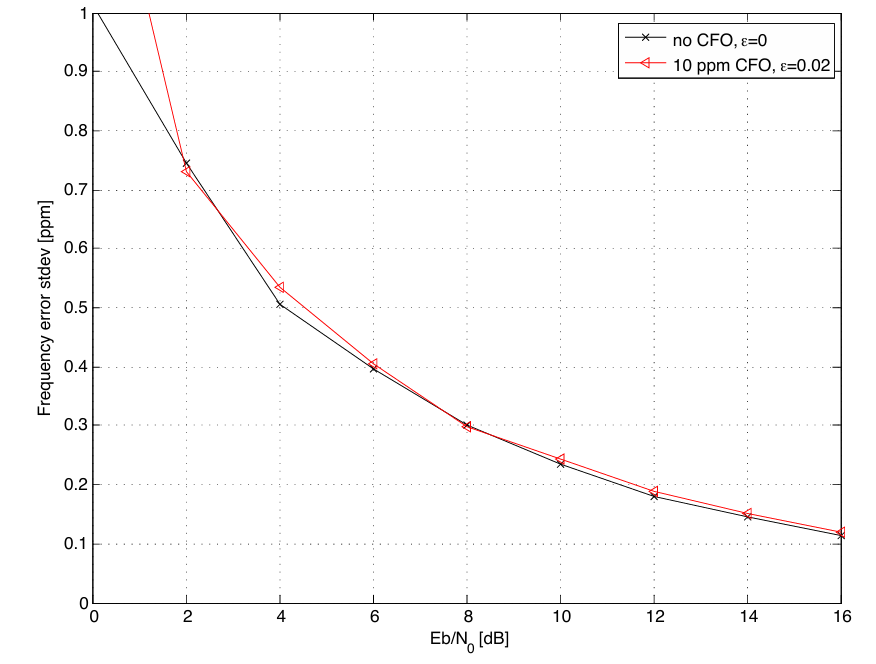
\includegraphics[width=0.8\textwidth]{time_frame_arrival_error_SNR.png}
    \caption{Frame time arrival standard deviation for realistic CFO and sampling time error based on SNR}
    \label{fig:time_frame_arrival_error_SNR}
\end{figure}